\documentclass[12pt,a4paper]{report}
% package de langues 
\usepackage[french]{babel}
\usepackage[utf8]{inputenc}
\usepackage[T1]{fontenc}

% package pour référence de liens sur pdf 
\usepackage[pdftex]{hyperref} % liens
\usepackage{lastpage} % numéro de page
\usepackage{caption}

% package de formes de document 
\usepackage[left=2.5cm,
              right=2.5cm,
              top=2.5cm,
              bottom=2.5cm
             ]{geometry}
% pour les tableaux 
\usepackage{array,multirow,makecell} 
\newcolumntype{R}[1]{>{\raggedleft\arraybackslash }b{#1}}
\newcolumntype{L}[1]{>{\raggedright\arraybackslash }b{#1}}
\newcolumntype{C}[1]{>{\centering\arraybackslash }b{#1}}

% package pour la page de couverture 
\usepackage{graphicx}
\usepackage[cyr]{aeguill}
\usepackage{fancyheadings}
\usepackage{amsmath}
\usepackage{amsfonts}
\usepackage{amssymb}
\usepackage{geometry}
\usepackage{eso-pic}
\usepackage{tikz}
\usetikzlibrary{calc}


% nouvelle commande pour la forme 
%\fancyhf[OFC]{\thepage / \pageref{LastPage}}
\rfoot{\thepage / \pageref{LastPage}}
%\setcounter{tocdepth}{3}

% pakages de couleurs du document
\usepackage{color}
\usepackage{xcolor}


% package pour la chimie
\usepackage[version=4]{mhchem}


% package pour la visualisation du code
\usepackage{listings}
\definecolor{darkWhite}{rgb}{0.94,0.94,0.94}
 
\lstset{
  aboveskip=3mm,
  belowskip=-2mm,
  backgroundcolor=\color{darkWhite},
  basicstyle=\footnotesize,
  breakatwhitespace=false,
  breaklines=true,
  captionpos=b,
  commentstyle=\color{red},
  deletekeywords={...},
  escapeinside={\%*}{*)},
  extendedchars=true,
  framexleftmargin=16pt,
  framextopmargin=3pt,
  framexbottommargin=6pt,
  frame=tb,
  keepspaces=true,
  keywordstyle=\color{blue},
  language=python,
  literate=
  {²}{{\textsuperscript{2}}}1
  {⁴}{{\textsuperscript{4}}}1
  {⁶}{{\textsuperscript{6}}}1
  {⁸}{{\textsuperscript{8}}}1
  {€}{{\euro{}}}1
  {é}{{\'e}}1
  {è}{{\`{e}}}1
  {ê}{{\^{e}}}1
  {ë}{{\¨{e}}}1
  {É}{{\'{E}}}1
  {Ê}{{\^{E}}}1
  {û}{{\^{u}}}1
  {ù}{{\`{u}}}1
  {â}{{\^{a}}}1
  {à}{{\`{a}}}1
  {á}{{\'{a}}}1
  {ã}{{\~{a}}}1
  {Á}{{\'{A}}}1
  {Â}{{\^{A}}}1
  {Ã}{{\~{A}}}1
  {ç}{{\c{c}}}1
  {Ç}{{\c{C}}}1
  {õ}{{\~{o}}}1
  {ó}{{\'{o}}}1
  {ô}{{\^{o}}}1
  {Õ}{{\~{O}}}1
  {Ó}{{\'{O}}}1
  {Ô}{{\^{O}}}1
  {î}{{\^{i}}}1
  {Î}{{\^{I}}}1
  {í}{{\'{i}}}1
  {Í}{{\~{Í}}}1,
  morekeywords={*,...},
  numbers=left,
  numbersep=10pt,
  numberstyle=\tiny\color{black},
  rulecolor=\color{black},
  showspaces=false,
  showstringspaces=false,
  showtabs=false,
  stepnumber=1,
  stringstyle=\color{gray},
  tabsize=4,
  title=\lstname,
}

%package pour les algorithmes
\usepackage{algorithm}
\usepackage{algorithmic}
\usepackage{amsmath}

% package pour les tableaux
\usepackage{longtable}
\usepackage{booktabs}

% package pour les figures 
\usepackage{subcaption}

% package de reférencement
% \usepackage[backend=biber,safeinputenc, sorting=none]{biblatex}

% mettre la bibliographie dans la table de matières
%\usepackage[nottoc, notlof, notlot]{tocbibind}
\include{page_couverture.tex}


\author{MBE MBE MINDJANA LOIC HENRI}
\title{GNPS et MDByTE}

\begin{document}
    
	\pagecouverture
	{Experimentations}
	{Apprentissage par ensemble Bagging}
	\tableofcontents
	\vspace{20cm}
    
	\section{Introduction}
	Dans le but de construire des groupes de molécules sur la base de leurs spectres RMN et MS, pour accélérer la recherche des médicaments basées sur les plantes naturelles, nous avons proposé deux algorithmes d'apprentissage par ensemble.

	Le premier utilise l'approche Bagging qui consiste à construire des échantillons aléatoirement de taille donnée, qui seront utilisés par des modèles de base pour construire des clusters, qui seront par la suite combinées par vote majoritaire. Le vote étant fait avec l'algorithme MCLA qui respecte clairement la définition de vote majoritaire.
	Le deuxième utilise l'approche Boosting, qui par contre construit les échantillons en sélectionnant progressivement les observations mal regroupées par les modèles de base, en utilisant les algorithmes tels que GNPS et ou MADByTE comme oracle de groupement.
    
	Pour pouvoir évaluer la pertinence des ces approches malgré les contraintes, nous avons évalué l'apprentissage par ensemble Bagging, sans intégrer GNPS et MADByTE dans le processus, qui est à cet effet sujet à ce document.
	Ce document se poursuivra en plusieurs étapes à savoir, la définition des hypothèses guidant notre expérimentation, la présentation des éléments d'expérimentations, puis l'analyse des paramètres dont la taille des échantillons et le nombre de weak-learners en passant par le fine tuning, et enfin la présentation des résultats d'expérimentation avec quelques observations.
    
	\section{Hypothèses d'expérimentations}
	Pour pouvoir évaluer et étendre la pertinence d'utiliser les approches proposés d'apprentissage, nous avons définit les hypothèses suivantes:
    
	\begin{itemize}
    	\item L'échantillonnage des observations améliore la qualité des clusters issus de l'apprentissage par ensemble par rapport au modèle de base
    	\item Combiner plusieurs algorithmes homogènes de clustering multi-vues, améliorerait la qualité des clusters
	\end{itemize}
    
	\section{Eléments d'expérimentations}
	Pour pouvoir mener à bien les expérimentations, nous avons utilisé un ordinateur portable ayant les caractéristiques suivante:
    
	\begin{itemize}
    	\item 8 CPUs (2.4Ghz de fréquence chacun)
    	\item 12 Go de mémoire
	\end{itemize}
    
	Nous les avons mené sur la dataset MSRC-V1 d'images qui contient 210 objets pour 7 classes. Les 7 classes correspondent à des arbres, des bâtiments, des avions, des visages, des voitures, des bœufs, des voitures et des bicyclettes. Cette dataset contient 210 objets, avec 4 vues qui correspondent à des caractéristiques extraites de ces images.

 	Comme métrique de performances, nous avons utilisé :
	\begin{itemize}
    	\item Exactitude (ACC) : qui permet de mesurer à quel point les clusters construits correspond à ceux de la réalité
    	\item Information Mutuelle normalisée (NMI) : qui permet de mesurer la quantité d'informations partagées entre les clusters construits et les clusters réels.
    	\item Pureté (PUR) : qui permet de mesurer le degré d'homogénéité des clusters construit par rapport aux groupes réelles
	\end{itemize}

	Nous avons exécuté tous les modèles 10 fois de suite et fait des moyennes de performances, pour le fine tuning, les analyses de paramètres et les expérimentations, dans le but de capturer leurs degrés d'instabilité.
    
	Comme modèle de base nous avons choisi MCLES et MVGL ( implémentés en python dû aux contraintes financières, avec les valeurs d’hyper-paramètres par défaut) , pour plusieurs raisons dont les plus importantes sont les suivantes :
	\begin{itemize}
    	\item ils sont très peu sensibles au biais des données d'origine
    	\item MCLES visent dans sa construction de cluster à construire la représentation unifiée des exemples
    	\item MVGL utilise des graphes de vues d'origine d'exemples dont il nettoie les biais avant leur fusion par pondération, ce qui faciliterait l'entrée des réseaux moléculaires
	\end{itemize}
    
	Pour pouvoir éviter qu'une observation ne trouve dans aucun échantillon, nous avons passé l'ensemble des observations au premier modèle de base.
    
	\section{Fine Tuning et Analyse des hyper-paramètres}
	Dans le but de donner des valeurs par défaut au nombre de weak-learners et à la taille des échantillons qui est vue en pourcentage du nombre d'exemples utilisés, nous avons fixé la grille de recherche avec :

	\begin{itemize}
    	\item Le nombre de weak-learner (nw) allant de 10 à 100 avec des écarts de 5
    	\item Le pourcentage utilisé des observations comme taille d'échantillons (p) allant de 50\% à 95\% avec des écarts de 5\%.
	\end{itemize}
    
    	\subsection{Fine-Tuning}
        	Nous avons exécuté l'apprentissage par ensemble en utilisant comme modèle de base MCLES, puis MVGL sur la grille donnée.
       	 
        	\subsubsection{Bagging avec MCLES}

        	Nous pouvons voir sur la figure \ref{fig:bagmcles_cor} issue de la sauvegarde des performances pour chaque couple de paramètres qu'on a:
        	\begin{itemize}
            	\item Une bonne corrélation entre la taille des échantillons et l'information mutuelle entre les clusters construits et les groupes réels
            	\item Une faible corrélation négative entre la taille des échantillons et l'exactitude du modèle
            	\item Une corrélation malheureusement pas très grande entre le nombre de weak-learners et la qualité des clusters construits, mais plus prononcée avec l'exactitude et la pureté
        	\end{itemize}
       	 
        	\begin{figure}
            	\centering
            	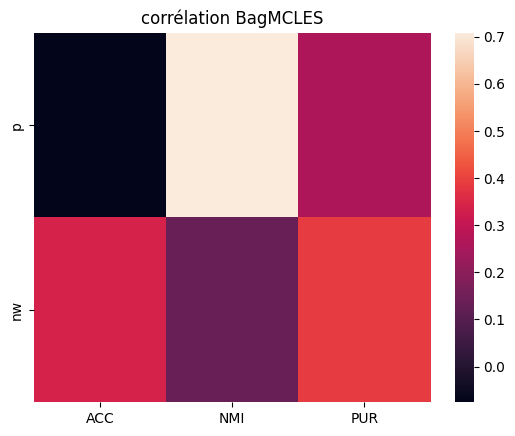
\includegraphics[width=0.5\linewidth]{Images/bagmcles_cor.png}
            	\caption{Corrélation entre les paramètres et les performances en utilisant MCLES comme weak-learner}
            	\label{fig:bagmcles_cor}
        	\end{figure}

        	Des mêmes données, on obtient la figure \ref{fig:bagmcles_corp} sur laquelle on voit, par rapport aux performances, qu'il y'a une forte corrélation négative entre la taille des échantillons et le nombre de weaks-learners utilisés
        	\begin{figure}
            	\centering
            	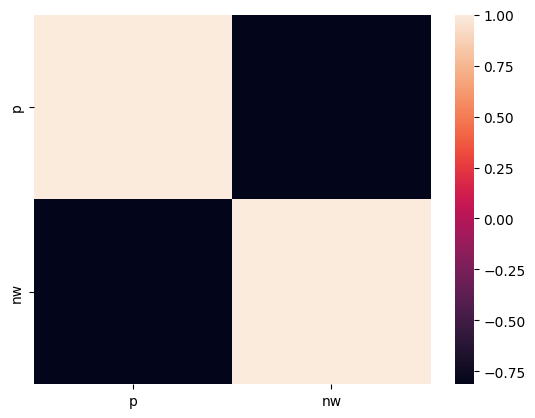
\includegraphics[width=0.5\linewidth]{Images/bagmcles_corp.png}
            	\caption{Corrélation entre les paramètres en utilisant MCLES comme weak-learner}
            	\label{fig:bagmcles_corp}
        	\end{figure}

        	\subsubsection{Bagging avec MVGL}

        	En utilisant MVGL comme weak-learner, Nous remarquons comme on peut le voir sur la figure \ref{fig:bagmvgl_cor} qu'on a :
        	\begin{itemize}
            	\item comme pour le cas de `Bagging MCLES`, une corrélation malheureusement pas très grande entre le nombre de weak-learners et la qualité des clusters construits, mais cette fois il y'a plutôt une corrélation plus prononcée avec l'information mutuelle
            	\item Une bonne corrélation entre la taille des échantillons et l'homogénéité des clusters construits par rapport à la réalité
            	\item La taille des échantillons a une corrélation négative pas très forte avec l'exactitude du modèle et l'information mutuelle, néanmoins plus prononcée avec l'information mutuelle
        	\end{itemize}

        	\begin{figure}
            	\centering
            	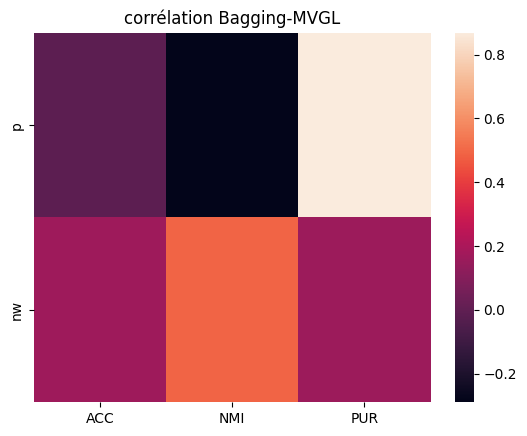
\includegraphics[width=0.5\linewidth]{Images/bagmvgl_cor.png}
            	\caption{Corrélation entre les paramètres et les performances en utilisant MVGL comme weak-learner}
            	\label{fig:bagmvgl_cor}
        	\end{figure}
       	 
        	De plus, nous avons toujours une forte corrélation négative entre ces hyper-paramètres \ref{fig:bagmvgl_corp}, malgré qu'elle est plus faible.
        	\begin{figure}
            	\centering
            	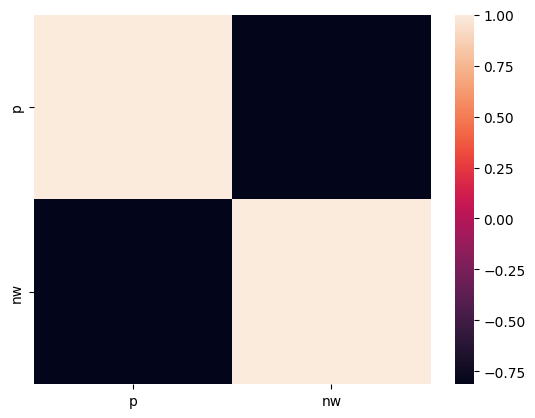
\includegraphics[width=0.5\linewidth]{Images/bagmcles_corp.png}
            	\caption{Corrélation entre les paramètres en utilisant MVGL comme weak-learner}
            	\label{fig:bagmvgl_corp}
        	\end{figure}


        	De ces remarques et des données, nous pouvons conclure que, augmenter le nombre de weak-learners et la taille des échantillons permet d'améliorer les performances du modèle.
        	Néanmoins puisqu'il y'a une corrélation négative entre ces deux paramètres, il faudra prioriser l'augmentation de l'un sur l'autre.

        	Nous pensons que donner la priorité à l'augmentation du nombre de weak-learners est plus profitable, car il est possible d'accélérer l'approche Bagging en le parallélisant (ce qui a été fait pour des besoins techniques), tout en ayant la certitude qu'il sera plus performant.
        	Il est d'autant plus important dans le cas où MVGL est weak-learner. Dans ce cas, nous avons des corrélations négatives, malgré qu'elles sont faibles, entre la taille des échantillons et les métriques d'exactitude et d'information mutuelle.

    	\subsection{Analyse individuel d'hyper-paramètres}
        	Au vue de l'analyse précédente, on a donné comme valeur par défaut au nombre de weak-learners à `100` (contraintes matérielle). Grâce à cela on a pu faire l'analyse sur la taille des échantillons, puis sur le nombre de weak-learners, en considérant les modèles de weak-learner étant MCLES et MVGL.
    
        	\subsubsection{Bagging avec MCLES}

        	Les courbes présentent dans la figure \ref{fig:bagmcles_pr} obtenue, permettent d'appuyer les observations qui ont été faites au niveau de l'analyse globale.
       	 
        	On peut voir que plus on augmente la taille des échantillons, plus on a tendance à avoir des clusters de moins en moins homogène, qui respectent de moins en moins la constitution des groupes réels. Néanmoins, cela augmente les informations communes avec ces groupes réels. De plus, plus on augmente le nombre de weak-learners, plus on construit les clusters homogènes respectant la constitution des groupes réels, sans pour autant augmenter les informations communes avec ces groupes.
       	 
        	\begin{figure}
       		 \centering
       		 \begin{subfigure}{0.4\linewidth}
       			 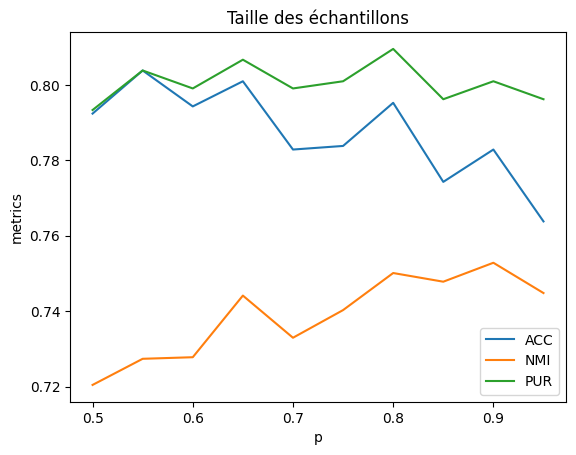
\includegraphics[width=\linewidth]{Images/bagmcles_p.png}
       			 \caption{Taille des échantillons}
       			 \label{fig:bagmcles_pr_p}
       		 \end{subfigure}
       		 \begin{subfigure}{0.4\linewidth}
       			 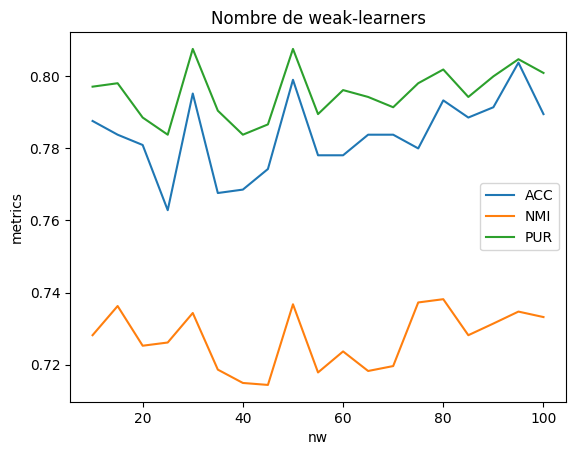
\includegraphics[width=\linewidth]{Images/bagmcles_nw.png}
       			 \caption{Nombre de weak-learner}
       			 \label{fig:bagmcles_pr_nw}
       		 \end{subfigure}
       		 \caption{Analyse de performance par rapport aux paramètres avec MCLES comme weak-learner}
       		 \label{fig:bagmcles_pr}
        	\end{figure}

            \begin{figure}
       		 \centering
       		 \begin{subfigure}{0.3\linewidth}
       			 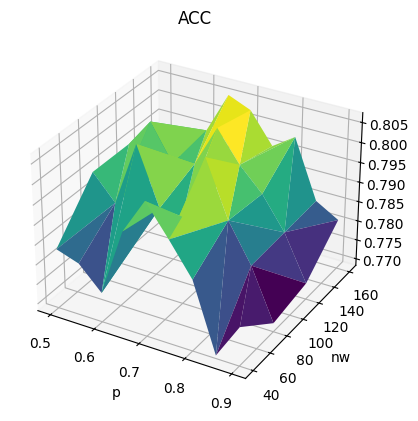
\includegraphics[width=\linewidth]{Images/ACC_mcles.png}
       			 \caption{ACC}
       			 \label{fig:bagmcles_acc}
       		 \end{subfigure}
              \begin{subfigure}{0.3\linewidth}
       			 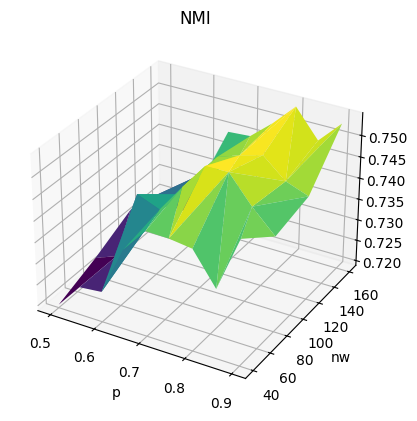
\includegraphics[width=\linewidth]{Images/NMI_mcles.png}
       			 \caption{NMI}
       			 \label{fig:bagmcles_nmi}
       		 \end{subfigure}
              \begin{subfigure}{0.3\linewidth}
       			 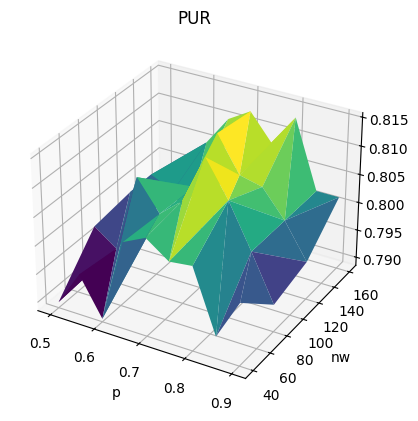
\includegraphics[width=\linewidth]{Images/PUR_mcles.png}
       			 \caption{PUR}
       			 \label{fig:bagmcles_pur}
       		 \end{subfigure}
       		 \caption{Graphes de performances de type Bagging avec MCLES}
       		 \label{fig:bagmcles_pr}
        	\end{figure}

            \begin{figure}
       		 \centering
       		 \begin{subfigure}{0.3\linewidth}
       			 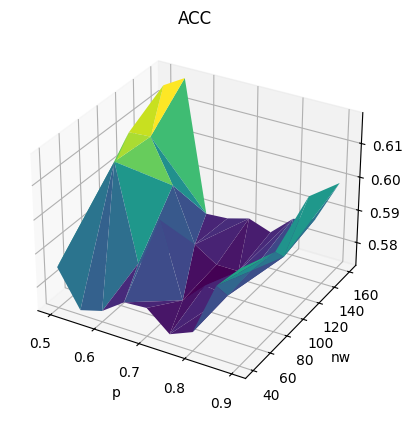
\includegraphics[width=\linewidth]{Images/ACC_mvgl.png}
       			 \caption{ACC}
       			 \label{fig:bagmcles_acc}
       		 \end{subfigure}
              \begin{subfigure}{0.3\linewidth}
       			 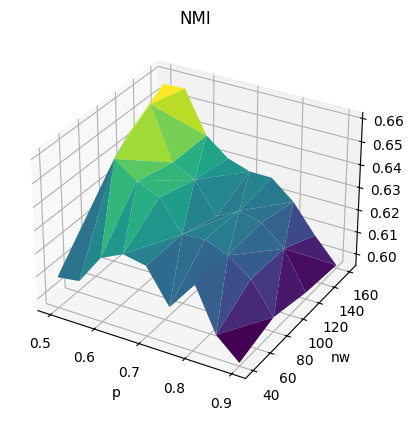
\includegraphics[width=\linewidth]{Images/NMI_mvgl.png}
       			 \caption{NMI}
       			 \label{fig:bagmcles_nmi}
       		 \end{subfigure}
              \begin{subfigure}{0.3\linewidth}
       			 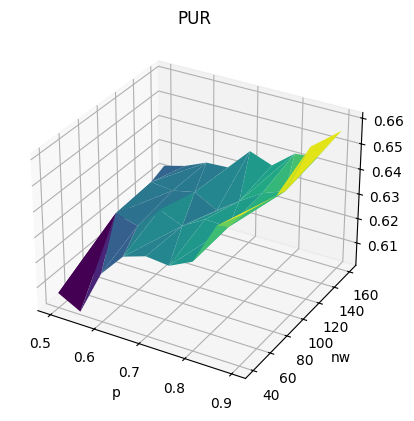
\includegraphics[width=\linewidth]{Images/PUR_mvgl.png}
       			 \caption{PUR}
       			 \label{fig:bagmcles_pur}
       		 \end{subfigure}
       		 \caption{Graphes de performances de type Bagging avec MVGL}
       		 \label{fig:bagmcles_pr}
        	\end{figure}

        	\subsubsection{Bagging avec MVGL}

        	Dans le cas où on utilise MVGL comme weak-learner, On obtient les courbes \ref{fig:bagmvgl_pr} qui valident encore plus les observations faites lors de l'analyse globale.

        	On peut voir que plus on augmente la taille des échantillons, plus on a des clusters homogènes, mais qui respectent de moins en moins la constitution des groupes réels. De plus, il y’a réduction de la quantité d’informations communes avec ces groupes réels. On remarque également que, plus on augmente le nombre de weak-learners, plus on construit des clusters de meilleure qualité.

        	\begin{figure}
       		 \centering
       		 \begin{subfigure}{0.4\linewidth}
       			 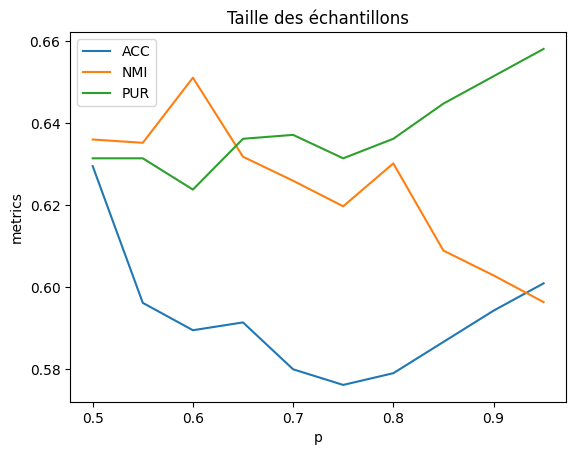
\includegraphics[width=\linewidth]{Images/bagmvgl_p.png}
       			 \caption{Taille des échantillons}
       			 \label{fig:bagmvgl_pr_p}
       		 \end{subfigure}
       		 \begin{subfigure}{0.4\linewidth}
       			 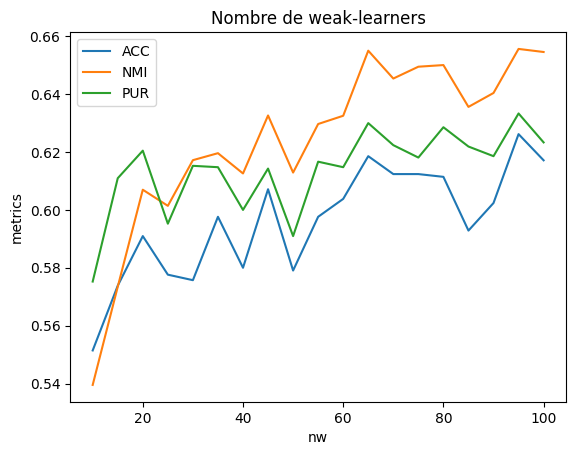
\includegraphics[width=\linewidth]{Images/bagmvgl_nw.png}
       			 \caption{Nombre de weak-learner}
       			 \label{fig:bagmvgl_pr_nw}
       		 \end{subfigure}
       		 \caption{Analyse de performance par rapport aux paramètres avec MVGL comme weak-learner}
       		 \label{fig:bagmvgl_pr}
        	\end{figure}

        	Grâce à nos observations précédentes, nous avons sélectionné des valeurs par défaut du modèle, pour la dataset `MSRC-V1` qui sont contenues dans le tableau \ref{table:default}, qui nous ont permis de passer à l'étape finale, qui constituent les expérimentations proprement dites.

        	\begin{table}[h!]
        	\caption{Tableau des valeurs par défaut du modèle}
        	\centering
            	\begin{tabular}{lcr}
                	\toprule
                 	& p & nw \\
                	\midrule
                	BagMCLES & 60\% & 100 \\
                	BagMVGL & 55\% & 100 \\
                	\bottomrule
            	\end{tabular}
        	\label{table:default}
        	\end{table}

	\section{Résultats d'expérimentations et analyse}
	En utilisant les paramètres par défaut données, nous avons réalisé les expérimentations, dont les résultats sont visibles au tableau \ref{table:perfs}.
    
	\begin{table}[h!]
    	\caption{Tableau des performances}
    	\centering
        	\begin{tabular}{lrrr}
        	\toprule
         	& ACC & NMI & PUR \\
        	model &  &  &  \\
        	\midrule
        	MVGL & 0.600$\pm$0 & 0.595$\pm$0 & 0.657$\pm$0 \\
        	BagMVGL & \textbf{0.626$\pm$0.007} & \textbf{0.667$\pm$0.009} & \textbf{0.627$\pm$0.005} \\
        	MCLES & 0.720$\pm$0.058 & 0.718$\pm$0.033 & 0.755$\pm$0.047 \\
        	BagMCLES & \textbf{0.803$\pm$0.020}& \textbf{0.733$\pm$0.012} & \textbf{0.806$\pm$0.015} \\
        	\bottomrule
        	\end{tabular}
    	\label{table:perfs}
	\end{table}
    
	Ce tableau nous permet de réaliser les éléments suivants:
	\begin{itemize}
    	\item Le modèle d'apprentissage par ensemble est plus performant que les modèles de base généralement
    	\item Si les weak-learners sont très stables (suivant ces performances), le modèle le sera aussi mais moins fortement, mais on pourra avoir des clusters moins homogènes
    	\item Si plutôt ils sont instables, le modèle sera encore plus stable et augmentera la qualité des clusters
	\end{itemize}
    
	Cela se justifie car MCLES n'est pas très stable surtout parce qu'il utilise l'algorithme Kmeans pour construire ces clusters. MVGL l'est bien moins vu qu'il calcule les clusters en considérant qu'ils sont des composantes connexes.
	De ce fait on peut émettre l'hypothèse que, orienter la construction des échantillons vers des exemples mal groupés pourrait augmenter les performances, car permettrait d'apprendre des structures complexes dans les données, qui empêchent la construction de meilleures clusters. Cela pourrait amener à se poser la question de l'importance de chacune des vues dans la construction des clusters.
    
	%est ce que pourrait modifier la construction de la représentation unifié de MCLES pour qu'il puisse fournir pour des exemples semblables contenus dans des échantillons différents, des représentations unifiés semblables
    
	\section{Conclusion}
	En somme, il était question pour nous d'évaluer l'approche d'apprentissage Bagging sur la base des métriques de performances telles que l'exactitude, l'information mutuelle normalisée et la pureté.

	Nous pensons au travers des résultats obtenus que les hypothèses ont été validées, et que l'approche Boosting pourrait être plus performant que celle du Bagging. Les performances montrent que MCLES capturent des structures complexes contenues dans les vues par rapport à MVGL, et que cela se vérifie également quand on les utilise comme modèle de base. 

Lors de ces expérimentations, nous avons eu principalement le problème de puissance de calcul, qui nous a amené à se poser la question de comment mieux et plus sérieusement accélérer l'apprentissage ?
    
%  \bibliographystyle{unsrt}
    \bibliography{reference_GNPS_MADByTE}
\end{document}
